%Tex root = ProbabilitàEStatistica.tex

\chapter{Laboratorio}

      \section{Introduzione ad R}

         R è stato avviato dai professori Ross Ihakae Robert Gentleman come linguaggio di programmazione 
per insegnare statistica introduttiva all’Universitàdi Auckland nel 1993.
\begin{itemize}
  \item Il linguaggio ha preso forte ispirazione dal linguaggio di programmazione S.
  \item Il Comprehensive R Archive Network(CRAN) è stato fondato nel 1997 da KurtHornik e FritzLeischper ospitare il codice sorgente di R, i file eseguibili, la documentazione e i pacchetti creati dagli utenti.
  \item In origine, CRAN aveva tre mirror e 12 pacchetti contribuiti. A dicembre 2022 conta 103 mirror e 18.976 pacchetti contribuiti
\end{itemize}

\subsection{Pacchetti importanti}
\begin{description}
  \item[\textbf{\underline{ggplot2:}}] per la visualizzazione dei dati 
  \item[\textbf{\underline{dplyr:}}] per la manipolazionedei dati, inclusi filtraggio, raggruppamento e sintesi dei dati
\item[\textbf{\underline{tidyr:}}] per pulire e ristrutturare i dati
\item[\textbf{\underline{caret:}}] per il machine learning
\item[\textbf{\underline{lubridate:}}] per lavorarecon date e orari
\item[\textbf{\underline{stringr:}}] per lavorarecon le stringhe, incluse funzioni per il pattern matching, la manipolazionedelle stringhe e le espressioni regolari
\item[\textbf{\underline{reshape2:}}] per trasformarei dati tra formati “wide” e “long”
\item[\textbf{\underline{data.table:}}]per la manipolazione e aggregazione dei dati, particolarmente utile per lavorare
condataset di grandi dimensioni

\end{description}

\textbf{\textcolor{black!50!red}{Per installare e utilizzare un pacchetto}}
\begin{codiceR}
  install.packages("package_name") # install the package 
  library("package_name") # load the package
\end{codiceR}


\section{Primi comandi}
Puoi eseguire comandi nella console di R, ad esempio per calcolare 
un’espressione matematica:

\begin{codiceR}
  > 1+1
  [1] 2
\end{codiceR}
Oppure scrivi la stessa espressione in un file script .R e poi premi <Ctrl> + Enter per inviare la riga selezionata alla console.\par

Puoi anche dichiarare variabili usando gli operatori <- o =
\begin{codiceR}
  > A <- 1+1 
> A
  [1] 2
\end{codiceR}

\subsection{Cronologia dei comandi}

In R, puoi vedere i comandi precedenti usando la freccia su nella console. Ogni 
pressione mostra il comando precedente,che puoi modificare o eseguire.
In alternativa, usa la funzione history() nella console o il   pannello History per accedere alla cronologia della sessione corrente.

\subsection{Ottenere aiuto (help)}
Per accedere alla documentazione di una funzione o di un pacchetto, digita nella console:
\texttt{?nome\_funzione} o \texttt{?nome\_pacchetto} e premi Enter

\begin{codiceR}
> #Get help for the mean() funcion
> ?mean
\end{codiceR}

\vario{Nota}{Usando la sintassi \texttt{??"search term"} ottieni una lista di tutte le pagine di aiuto che contengono il termine}

In alternativa è possibile usare: help(function\_name) or help (package\_name)
\begin{codiceR}
> # This time get help using help() function
> help(mean)
\end{codiceR}
In uno script.R premendo <Ctrl> + F1 con il nome di una funzione selezionato si apre la relativa documentazione.

Il pannello Help mostra tutte le informazioni disponibili. Se non basta, esistono molte risorse online

\section{Variabili semplici}
Quando
vuoi memorizzare il risultato di un calcolo per riutilizzarlo o dargli un nome sensato per
rendere il codice più leggibile, definisci una variabile

\subsection{Assegnazione, Sovrascrittura, Rimozione}

\textbf{\large Assegnazione}
\begin{codiceR}
  > students <- 100
\end{codiceR}
Creata variabile students di tipo numerico. Il valore 100 viene memorizzato

\textbf{\large Sovrascrittura}
\begin{codiceR}
  > students <- 102
> students
  [1] 102
\end{codiceR}
Si può controllare il contenuto digitando il nome della variabile nella console o guardando il pannello environment

\textbf{\large Rimozione variabili}
\begin{codiceR}
  > remove(students)      #Removes a single variabile
> remove (list = ls())  # Removes all the variables listed by the ls() function
\end{codiceR}

\section{Vettori}
Un vettore in R è una lista di elementi

\textbf{\large Creazione}
\begin{codiceR}
  > v1 <- c(2, 5, 1)
\end{codiceR}
Creazione di un vettore numerico contenente 3 elementi

\textbf{\large Accedere agli elementi di un vettore}
\begin{codiceR}
  > v1[1]   #La parentesi quadra indica l'indice di interesse
  [1] 2
\end{codiceR}
L'indicizzazione parte da 1

\textbf{\large Creazione vettore come unione di più vettori}
\begin{codiceR}
  > r <- c(2, 4, 10)
> w <- c(9, -6, 4)
> u <- c(r, w)
  [1] 2 4 10 9 -6 4
\end{codiceR}

\textbf{Operatore due punti}
\begin{codiceR}
  > x1 <- 1:10
> x1
  [1] 1 2 3 4 5 6 7 8 9 10
\end{codiceR}
L'operatore due punti genera un vettore di elementi regolarmente distribuiti

\textbf{Funzione seq()}
Per creare sequenze più specifiche si usa la funzione \textbf{seq()}

\begin{codiceR}
  > x2 <- seq(from = 0, to = 0.5, by = 0.1)
> x2
  [1] 0.0 0.1 0.2 0.3 0.4 0.5
\end{codiceR}

\textbf{Funzioni correlate}
\begin{itemize}
  \item seq\_along(): crea un vettore con tanti elementi quanti quelli del vettore passato tra parentesi
  \item seq\_len(): crea un vettore con tanti elementi quanti indicati da un argomento intero
\end{itemize}


\subsection{Ripetizioni di vettori}
\begin{codiceR}
  > r1 <- rep(c(1,2,3), times = 3)
> r1
  [1] 1 2 3 1 2 3 1 2 3
\end{codiceR}
Esempio: il vettore 1, 2, 3 ripetuto 3 volte

Per ripetere \textbf{ogni elemento} un numero specifico di volte, usa gli argomenti di rep()

\begin{codiceR}
  > r2 <- rep(c(1,2,3), each = 3)
> r3 <- rep(c(1,2,3), times = c(1,2,3))
> r2
  [1] 1 1 1 2 2 2 3 3 3
> r3
  [1] 1 2 2 3 3 3

\end{codiceR}

\subsection{Funzioni utili per i vettori}
\begin{description}
  \item[length():] Restituisco la lunghezza del vettore
  \item[max(), min():] Calcola il valore massimo e minimo
  \item[sum():] Somma tutti gli elementi
  \item[mean():] Calcola la media
  \item[cumsum():] Calcola la somma cumulativa di ogni elemento 
\end{description}

\section{Matrici}
\textbf{\large Come creare una matrice:}
\begin{itemize}
  \item concatenando vettori come colonne (funzione \textbf{cbind})
  \item concatenando vettori come righe (funzione \textbf{rbind})
  \item usando la funzione \textbf{matrix()}, specificando numero di righe e colonne
\end{itemize}

\begin{codiceR}
  > mat1 <- cbind(c(1,2,3), c(4,5,6))
> mat2 <- rbind(c(1,2,3), c(4,5,6))
> mat3 <- matrix(data = c(1,2,3,4,5,6), nrow = 3, ncol = 2)
\end{codiceR}


\begin{figure}[H]
    \centering % Centra l'intera figura principale sulla pagina
    % --- PRIMA FOTO ---
    \begin{subfigure}[b]{0.3\textwidth} 
        \centering
        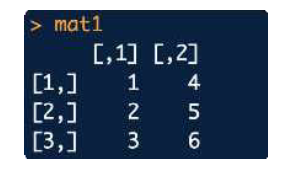
\includegraphics[width=\textwidth]{images/mat1.png} 
    \end{subfigure}
    \hfill
    % --- SECONDA FOTO ---
    \begin{subfigure}[b]{0.3\textwidth} 
        \centering
        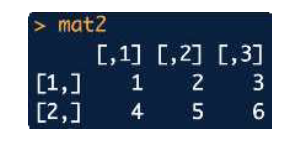
\includegraphics[width=\textwidth]{images/mat2.png}
    \end{subfigure}
    \hfill
    % --- TERZA FOTO ---
    \begin{subfigure}[b]{0.3\textwidth}
        \centering
        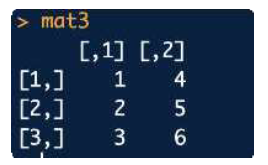
\includegraphics[width=\textwidth]{images/mat3.png}
    \end{subfigure}

\end{figure}

\textbf{\large Accedere agli elementi}\\
Per accedere agli elementi della matrice servono due indici, uno per le righe e uno per le colonne.
\begin{codiceR}
  > mat1 <- cbind(c(1,2,3), c(4,5,6))
>mat2[2,2] #element in second row, second column
  [1] 5
\end{codiceR}

Per ottenere tutti gli elementi di una riga o colonna bisogna lasciare vuoto l'indice opposto

\begin{codiceR}
  > mat1[,2] #elementi della seconda colonna
  [1] 4 5 6
> mat2[2,] #elemnti della seconda riga
  [1] 2 5
\end{codiceR}

\textbf{\large Selezionare sottoinsieme di righe e colonne}
\begin{codiceR}
  > mat1 <- cbind(c(1,2,3), c(4,5,6))
> mat1[2:3, 1:2]    #seconda e terza riga, entrambe le colonne
        [,1][,2]
  [1,]  2     5
  [2,]  3     6
\end{codiceR}
Lo stesso approccio può essere utilizzato per i vettori. Gli indici degli elementi da rimuovere sono preceduti da un simbolo meno.

\subsection{Matrici speciali}
Esistono matrici particolari come matrici nulle, identità o diagonali


\begin{codiceR}
  > mat_zero <- matrix(0, 3, 3)   #Matrice 3x3 di zeri
> mat_ones <- matrix(1,3, 3)  #Matrice 3x3 di uno
> mat_id <- diag(3)   #Matrice identita 3x3
\end{codiceR}


\begin{figure}[H]
    \centering 
    % --- PRIMA FOTO ---
    \begin{subfigure}[b]{0.3\textwidth}
        \centering
        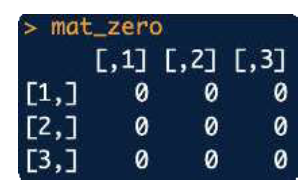
\includegraphics[width=\textwidth]{images/zeros.png} 
    \end{subfigure}
    \hfill 
    % --- SECONDA FOTO ---
    \begin{subfigure}[b]{0.35\textwidth}
        \centering
        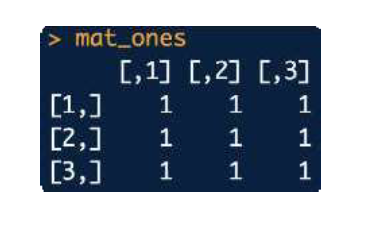
\includegraphics[width=\textwidth]{images/ones.png}
    \end{subfigure}
    \hfill 
    % --- TERZA FOTO ---
    \begin{subfigure}[b]{0.3\textwidth}
        \centering
        
\includegraphics[width=\textwidth]{images/ids.png}
    \end{subfigure}

\end{figure}

\subsection{Operazioni con vettori e matrici}
Le operazioni aritmetiche come somma, sottrazione, moltiplicazione e divisione vengono eseguite elemento per elemento

\begin{codiceR}
  > A <- matrix(data = 1:9, nrow = 3)
> B <- A +1
\end{codiceR}




\begin{figure}[h] % Ambiente figura principale. [htbp] suggerisce la posizione.
    \centering % Centra l'intera figura principale sulla pagina
    % --- PRIMA FOTO ---
    \begin{subfigure}[b]{0.45\textwidth}
        \centering
        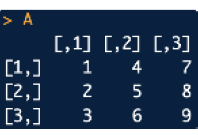
\includegraphics[width=0.85\textwidth]{images/A.png} 
        \caption{matrice A}
    \end{subfigure}
    \hfill 
    % --- SECONDA FOTO ---
    \begin{subfigure}[b]{0.45\textwidth}
        \centering
        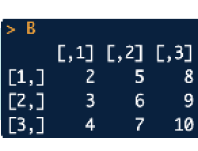
\includegraphics[width=0.85\textwidth]{images/B.png}
        \caption{matrice B (elementi A+1)}
      \end{subfigure}

\end{figure}


Altre operazioni elemento per elemento sono \textbf{l'elevamento a potenza} e la \textbf{radice quadrata}

\begin{codiceR}
  > C <- A^2
> D <- sqrt(A)
\end{codiceR}

\begin{figure}[H] % Ambiente figura principale. [htbp] suggerisce la posizione.
    \centering % Centra l'intera figura principale sulla pagina
    % --- PRIMA FOTO ---
    \begin{subfigure}[b]{0.45\textwidth}
        \centering
        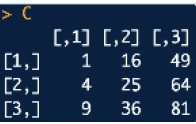
\includegraphics[width=0.85\textwidth]{images/C.png} 
      
    \end{subfigure}
    \hfill 
    % --- SECONDA FOTO ---
    \begin{subfigure}[b]{0.45\textwidth}
        \centering
        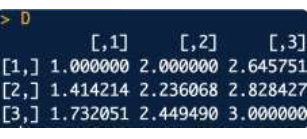
\includegraphics[width=0.85\textwidth]{images/D.png}
    \end{subfigure}

\end{figure}



Per ottenere statistiche riepilogative è possibile utilizzare le funzioni \textbf{sum()}, \textbf{mean()}, \textbf{max()}
\begin{codiceR}
  > sum(A)    #45       > min(A)   #1
> mean(A)   #5        > max(A)   #9    
\end{codiceR}

Le operazioni elemento per elemento possono essere eseguite anche tra matrici (purchè siano conformi tra loro)

\begin{codiceR}
  > A <- matrix(data = 1:9, nrow = 3)   #3x3
> E <- matrix(data = 1:4, nrow = 2)   #2x2
> A + E 
Error in A + E : non-conformable arrays
\end{codiceR}

Le operazioni tra matrici seguono le regole dell'algebra lineare (cioè la dimnesione e la forma necessarie degli input in relazione tra loro dipendono dall'operazione). \par
L'operatore \%*\% esegue la moltiplicazione tra matrici, mentre la funzione \textbf{t()} calcola la trasposta




\begin{figure}[H]
    \centering % Centra l'intera figura principale sulla pagina
    % --- PRIMA FOTO ---
    \begin{subfigure}[b]{0.3\textwidth} 
        \centering
        \begin{codiceR}
> v1 <- c(1,2,3)
> v2 <- c(4,5,6)
> v1 * v2
[1] 4 10 18
#Still element-wise
        \end{codiceR} 
    \end{subfigure}
    \hfill
    % --- SECONDA FOTO ---
    \begin{subfigure}[b]{0.3\textwidth} 
        \centering
        \begin{codiceR}
> t(v1) %*% v2
[1] 32
        \end{codiceR}
    \end{subfigure}
    \hfill
    % --- TERZA FOTO ---
    \begin{subfigure}[b]{0.3\textwidth}
        \centering
\begin{codiceR}
> v1 %*% t(v2)
      [,1][,2][,3]
[1,]    4   5   6
[2,]    8   10  12
[3,]    12  15  18
\end{codiceR}

    \end{subfigure}

\end{figure}



\begin{codiceR}
> v1 %*% t(v2)
      [,1][,2][,3]
[1,]    4   5   6
[2,]    8   10  12
[3,]    12  15  18
\end{codiceR}



\subsection{Funzioni utili per le matrici}

\begin{description}
  \item[det():] Restituisce il determinante di una matrice
  \item[qr():] Calcola la decomposizione QR 
  \item[solve()] Inversa di una matrice
  \item[nrow(), ncol():] Restituisce il numero di righe e di colonne
  \item[rowSums(), colSums():] Restituisce la somma di tutti gli elementi per riga o per colonna
  \item[rowMeans(), colMeans():] Restituisce la media di ogni riga o di ogni colonna
  \item[dim():] Restituisce il numeri di righe e colonne
\end{description}


\section{Caratteri}
Le variabili di tipo character servono per memorizzare testo.
\begin{codiceR}
  > month <- "March" #testo contenuto tra "" o ''
\end{codiceR}
Viene creata una variabile chiamata \textbf{month} che contiene la stringa "March"

\subsection{ Funzioni utili}
\begin{description}
  \item[nchar():] Restituisce la lunghezza di una stringa
  \item[paste(), paste0()] Unisce (concatena) due o più stringhe con o senza spazio
  \item[toupper():] Converte il testo in maiuscolo o minuscolo 
\end{description}

Come per i vettori numerici, è possibile creare vettori di caratteri
\begin{codiceR}
  > months <- c("january", "february", "march")
\end{codiceR}



\section{Liste, Array e Data Frame}

Le liste, gli array e i data frame sono tra i tipi di dati più flessibili in R.
\subsection{Liste}
Una lista è una collezione di dati che possono essere:
\begin{itemize}
  \item dello stesso tipo
  \item di tipi diversi
\end{itemize}


\subsection*{Creazione}

Per creare una lista si usa la funzione \texttt{list()}

\begin{codiceR}
> l1 <- list("Everest", "Nepal", 8848, TRUE)
> l2 <- list(81, 82, 90, 56)
\end{codiceR}
l1 contiene valori character, numerici e booleani, l2 contiene solo valori numerici

\subsection*{Come accedere}

\begin{codiceR}
> l1[1]
[[1]]
[1] "Everest"
\end{codiceR}
Accedere agli elementi di una lista è molto simile ai vettori

\subsection{Array}

Un array è una struttura di dati che può memorizzare dati dello stesso tipo in più di due dimnesioni.

\begin{itemize}
  \item \textbf{Vettori} $\rightarrow$ una dimensione
  \item \textbf{Matrici} $\rightarrow$ due dimensioni
  \item \textbf{Array} $\rightarrow$ più dimensioni
\end{itemize}


\begin{codiceR}
> a1 <- array(c(1:12), dim = c(2,3,2))
> a1
, , 1
      [,1]  [,2]  [,3]
[1,]    1     3     5
[2,]    2     4     6


, , 2
      [,1]  [,2]  [,3]
[1,]    7     9     11
[2,]    8    10     12
\end{codiceR}

\vario{Accesso agli elementi di un array}{In un array R, a1[i, j, k] indica l'elemento alla i-esima posizione della prima dimensione (righe), j-esima della seconda dimensione (colonne) e k-esima della terza dimensione (livello / profondità)}

\subsection{Data-Frame}
Un data frame è una \textbf{struttura di dati} \textbf{bidimensionale} che permette di memorizzare dati in forma tabellare.
I data frame hanno righe e colonne, e ogni colonna può essere un vettore diverso. \underline{I vettori possono anche avere tipi di dati differenti}.

\begin{codiceR}
> df1 <- data.frame(
      mount = c("Everest", "K2", "Fuji"),
      height = c(8848, 8611, 3776),
      todo = c(TRUE, TRUE, FALSE))
> df1
    mount height  todo
1 Everest   8848  TRUE
2      K2   8611  TRUE
3    Fuji   3776 FALSE
> df1$mount #Accedere ad una colonna  $
[1] "Everest" "K2" "Fuji"
\end{codiceR}



\subsection*{Concatenazione}
Si usano le funzioni \texttt{cbind()} e \texttt{rbind()} per unire due data frame orizzontalmente o verticalmente

\subsection*{Accesso}
\texttt{df1\$mount, df1[, "mount"]} e \texttt{df1[, 1]} sono modi equivalenti per accedere alla prima colonna del data frame

\section{Fattori}
Un \textbf{factor} è una struttura di dati utilizzata per lavorare con \textbf{dati categorizzabili}.
La funzione factor() può essere usata per creare un factor.
Una volta creato, un factor può contenere solo un insieme di valori predefiniti chiamati livelli(levels)-l
e categorie uniche




\begin{codiceR}
> f1 <- marital_status <- factor(c("married", "single", "single", "divorced", "married"))
> f1
[1] married single single divorced married
Levels: divorced married single
> levels(f1)
[1] "divorced" "married" "single"
> f1[1] <- "hey"
Warning message:
In '[<-.factor'('*tmp*', 1, value = "hey") :
  invalid factor level, NA generated]

\end{codiceR}

\subsection{Strutture  if, else}

\subsection*{Costrutto if-else}
Effettua un blocco di codice solo se la condizione è vera
\begin{codiceR}
  if (condizione){
    # istruzione
  } else if (condizione) {
    # istruzione
  }
\end{codiceR}

\subsection*{Costrutto ifelse}
Controlla una condizione per ogni elemento di un vettore e resistuisce valori diversi secondo il risultato.
\begin{codiceR}
  ifelse(condizione, yes = ..., no = ...)

> #Esempio
> voti <- c(6,9,10)
> ifelse(voti > 8, yes = "Ottimo", no = "Sufficiente")
[1] "Sufficiente" "Ottimo "Ottimo"
\end{codiceR}

\subsection{Struttura for, while}
Ripete un blocco di codice per ogni elemento di una sequenza o vettore

\begin{codiceR}
  for(variabile in vettore){
    #istruzione ripetute per ogni elemento del vettore
  }
\end{codiceR}

Cotrolla una condizione per ogni elemento di un vettore e restituisce valori diversi secondo il risultato.

\begin{codiceR}
while(condizione){
  # istruzione ripetute finche la condizione e' TRUE
}
\end{codiceR}


\section{Rappresentazione Grafica}
Per creare un grafico si può usare la funzione plot() integrata in R.

\subsection*{Esempio di grafico a dispersione(scatterplot)}


\begin{figure}[H]
    \centering 
    \begin{subfigure}[b]{0.45\textwidth} 
      \centering  
      \begin{codiceR}
  x <- c(1,2,3,4,5)
y <- c(2,4,6,8,10)

# Crea un scatterplot
plot(x,y)
\end{codiceR}
    \end{subfigure}
    \hfill
    % --- SECONDA FOTO ---
    \begin{subfigure}[b]{0.45\textwidth} 
        \centering
        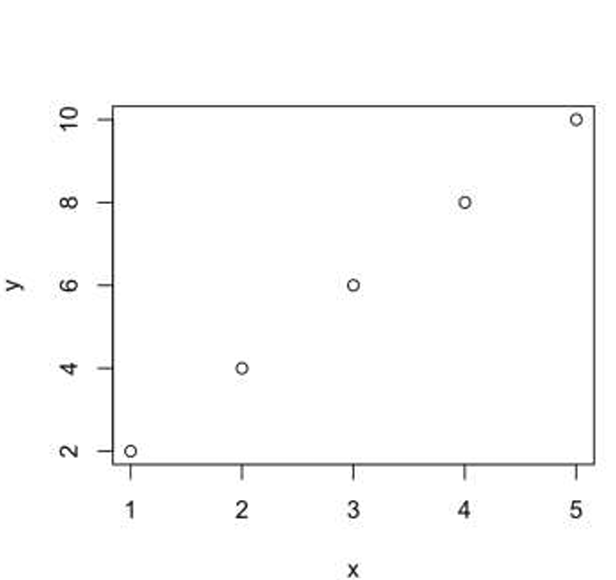
\includegraphics[width=\textwidth]{images/esempioScatterPlot.png}
    \end{subfigure}

\end{figure}




\subsection*{Tipologie di grafici}
\begin{description}
  \item[BarPlot:] I grafici a barre sono usati per visualizzare dati categorici. Ogni varra rappresenta una categoria e l'altezza della barra rappresenta la frequenza o proporzione di quella categoria.
  \item[Grafici a linee:] Usati per mostrare tendende o variazioni nel tempo
  \item[Istogrammi(hist()):] usati per mostrare la distribuzione di una variabie continua. L'asse X rappresenta l'itnervallo di valori e l0asse Y rappresenta la frequenza o propozione dei valor idi ciascun intervallo.
  \item[BoxPlot:] Usati per visualizzare la distribuzione di una variabile continua.
  \item[Grafici a dispersione:] Usati per mostrare la relazione tra due variabili continue, dove ogni punto dati è rappresentato da un punto su un grafico bidimensionale
  \item[Grafici di densità: ]Usati per visualizzare la distribuzione continua tramite uan curva liscia.     
\end{description}

\subsection{Grafico a Barre}
Usando il comando \texttt{plot(..., type = "l"):}

\begin{figure}[htbp]
    \centering 
    \begin{subfigure}[b]{0.45\textwidth} 
      \centering  
\begin{codiceR}[unbreakable, listing options={style=Rstyle, basicstyle=\ttfamily\footnotesize}]
ages = 20:29
students = c(2,1,5,3,4,2,0,2,1,0)
barplot(students,
xlab = "Age of students",
ylab = "Number of students", 
names.arg = ages)
\end{codiceR}
    \end{subfigure}
    \hfill
    % --- SECONDA FOTO ---
    \begin{subfigure}[b]{0.45\textwidth} 
        \centering
        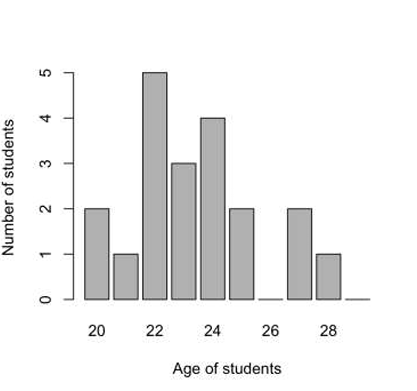
\includegraphics[width=\textwidth]{images/barplotto.png}
    \end{subfigure}
\end{figure}


\vspace{2em}

\subsection{Line Plot}
Usando il comando \texttt{plot(..., type = "1"):}


\begin{figure}[htbp]
    \centering 
    \begin{subfigure}[b]{0.55\textwidth} 
      \centering  
      \begin{codiceR}
> #Genera 100 valori casuali tra 10 e 20

daily_income <- runif(100, min = 10, max = 20)

plot(daily_income, 
    type = "1", 
    xlab = "Day",
    ylab = "Daily Income",
    main = "Daily incomes over 100 days")
\end{codiceR}
    \end{subfigure}
    \hfill
    % --- SECONDA FOTO ---
    \begin{subfigure}[b]{0.40\textwidth} 
        \centering
        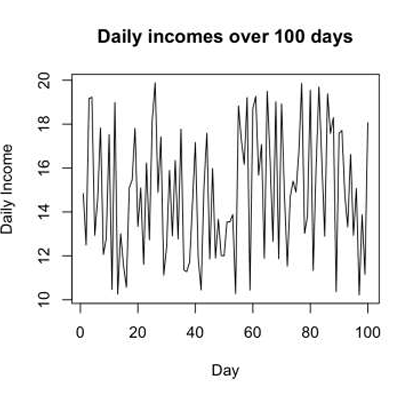
\includegraphics[width=\textwidth]{images/LinePlot.png}
    \end{subfigure}
\end{figure}


\subsection{Istogramma}
Usando il comando \texttt{hist():}




\begin{figure}[H]
    \centering 
    \begin{subfigure}[b]{0.55\textwidth} 
      \centering  
      \begin{codiceR}
> #Genera 100 valori casuali tra 40 e 80

weights <- runif(100, min = 40, max = 80)
> #In R, per vedere i primi elementi di un vettore, puoi usare la funzione head()

head(weights)

hist(weights, breaks = c(40,50,60,70,80))

\end{codiceR}
    \end{subfigure}
    \hfill
    % --- SECONDA FOTO ---
    \begin{subfigure}[b]{0.40\textwidth} 
        \centering
        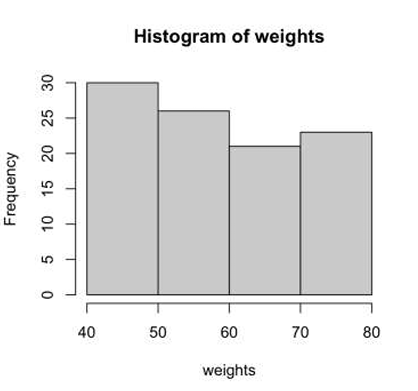
\includegraphics[width=\textwidth]{images/Istogramma2.png}
    \end{subfigure}
\end{figure}

\subsection{BoxPlot}
Usando il comando \texttt{boxplot():}

\begin{figure}[htbp]
    \centering 
    \begin{subfigure}[b]{0.55\textwidth} 
      \centering  
      \begin{codiceR}
> #Genera 50 valori causali tra 40 e 80
> #Genera 50 valori casuali tra 45 e 70

> height <- c(runif(50, min = 40, max = 80),
    runif(50, min = 45, max = 70))
> group <- rep(c("A", "B"), each = 50)

> boxplot(height ~ group, main = "Heights by group boxplots")
\end{codiceR}
    \end{subfigure}
    \hfill
    % --- SECONDA FOTO ---
    \begin{subfigure}[b]{0.40\textwidth} 
        \centering
        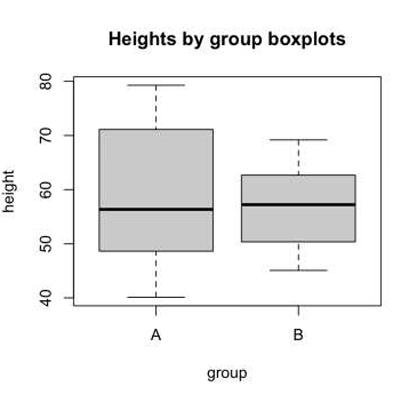
\includegraphics[width=\textwidth]{images/BoxPlot.png}
    \end{subfigure}
\end{figure}



\subsection{Mostrare più grafici contemporaneamente}
Usando il comando \texttt{par(mfrow = C(nrighe, ncolonne))} è possibile impostare il layout per più grafici



\begin{figure}[H]
    \centering 
    \begin{subfigure}[b]{0.55\textwidth} 
      \centering  
      \begin{codiceR}
> #Definire dei dati
> x = 1:6
> y = c(33,11,5,9,22,30)
> #Impostare il layout, 2 righe e 2 colonne
> par(mfrow = c(2,2))
> #Posizione [1,1]
> barplot(y, main = "Barplot", names.arg = x)
> #Posizione [1,2]
> barplot(y, main ="Horizontal Barplot", names.arg = x, horiz = TRUE)
> #Posizione [2,1]
> plot(x, y, type = "l", main ="Line plot")# Posizione [2, 2]

> plot(x, y, main = "Scatter plot", col = "red")

\end{codiceR}
    \end{subfigure}
    \hfill
    % --- SECONDA FOTO ---
    \begin{subfigure}[b]{0.40\textwidth} 
        \centering
        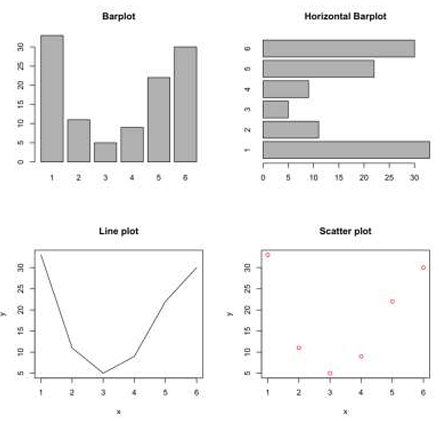
\includegraphics[width=\textwidth]{images/piùGraficiContemporaneamente.png}
    \end{subfigure}
\end{figure}

\subsection{Salvare ed esportare grafici}
Per salvare un grafico, è possibile usare le funzioni \texttt{pdf(), jpeg(), svg()} per creare un nuovo dispositivo grafico e poi usare la funzione \texttt{plot()} per creare il grafico
Una volta creato il grafico, puoi usare la funzione \texttt{dev.off()} per chiudere il dispositivo grafico e salvare il grafico in un file.

\begin{codiceR}
> #Crea un nuovo dispositivo grafico pdf
> pdf("./plots/myplot.pdf")
> #Qui bisogna indicare la directory dove salvare il file
> #Crea un grafico
  x <- 1:10
  y <- y^2
  plot(x,y)
> #Chiudi il dispositivo grafico e salva il grafico nel file
  dev.off()
\end{codiceR}


\section{Salvare e caricare}
\subsection{variabili}

Le variabili in R possono essere salvate utilizzando due formati principali: 
\begin{itemize}
  \item \textbf{.RData} è usato per salvare uno o più oggetti in un unico file. \begin{itemize}
    \item Salvare: \texttt{save()}
    \item Caricare: \texttt{load()}
  \end{itemize}
  \item \textbf{.RDS} è un formato usato per salvare un singolo oggetto R in un file
  \begin{itemize}
    \item Salvare: \texttt{saveRDS()}
    \item Caricare: \texttt{readRDS}
  \end{itemize}
\end{itemize}


\subsection{Dati Tabulari}
Spesso i dati da importare o esportare sono organizzati in formato tabellare.
Ci sono diverse opzioni:

\begin{itemize}
  \item \texttt{read.csv()/write.csv() e read.table() / write.table()}
  \item \texttt{read\_excel() / write\_excel()} dal pacchetto \texttt{readxl}: importare o esportare dati da/verso file Excel
  \item \texttt{readr::read\_delim()/write\_delim()} e \texttt{readr:read\_csv()/write\_csv():} utilizzate per importare o esportare da file di testo delimitati inclusi \textbf{CSV, TSV ...}
\end{itemize}



\section{File.R - script e funzioni}

Gli script e le funzioni sono due componenti che permettono di scrivere e riutilizzare codice:
\begin{itemize}
  \item \textbf{Script}: è un file di testo contenente una sequenza di comandi R che si desidera seguire. Oer eseguirli si utiziza la funzione \texttt{source()}
  \item \textbf{Funzione}: è un blocco di codice che svolge un compito specifico e può essere irchiamato da altre parti del codice. Le funzioni in R si definiscono usando \texttt{function()}
  
  \begin{codiceR}
    my_sum <- function(x,y){
      z <- x + y
      return(z)
      }
  #Esempio di funzione semplice
  \end{codiceR}
  Le variabili create all'interno di una funzione sono locali alla funzione (esistono solo mentre viene eseguita)

  \begin{codiceR}
    my_sum(2,3) #Restituisce 5
  \end{codiceR}
\end{itemize} 


\subsection{Variabili locali e gloabali}
Una variabile globale è una variabile definita al di fuori di qualsiasi funzione o blocco di codice e può essere accessibile da qualsiasi parte del programma.

\begin{codiceR}
  x <- 10
  my_function <- function(){
    y <- x+1
    return(y)
  }
  my_function() #Restituisce 11
\end{codiceR}


\vario{Nota}{Se si definisce una variabile con lo stesso nome all'interno di una funzione come una variabile glovale, la variabile globale avrà la precedenza e quella globale sarà mascherata all'interno della funzione}




\section{Statistica Descrittiva}

La statistica descrittiva è un settore della statistica che riguarda la raccolta, l’organizzazione, la sintesi e la presentazione dei dati. Fornisce un modo per descrivere e riassumere le caratteristiche di un insieme di dati, come la tendenza centrale, la dispersione, la forma e la distribuzione.

Le statistiche descrittive possono essere utilizzate per ottenere informazioni sui dati. Ad esempio, possiamo usarle per determinare l’età media di un gruppo di persone, la variabilità delle loro età e come queste sono distribuite all’interno del gruppo.

Quando un dataset contiene più di una variabile, a seconda del loro tipo (ad esempio discreta, continua, categorica…), le statistiche descrittive possono essere utilizzate per studiare le associazioni tra queste variabili (ad esempio covarianza e correlazione).

La visualizzazione aiuta a rendere più evidenti i pattern e le tendenze nei dati e può fornire una comprensione più intuitiva rispetto a una semplice tabella di numeri. Alcuni tipi comuni di visualizzazione includono grafici a dispersione, grafici a barre, grafici a linee e istogrammi.

\subsection{Funzioni comuni}
\begin{itemize}
  \item \textbf{mean()}: Media calcola il valore medio di un dataset
  \item \textbf{median()}: Mediana calcola il valore centrale di un dataset
  \item \textbf{range()}: Calcola l’intervallo tra il valore minimo e il massimo
  \item \textbf{IQR()}: Intervallo interquartile: misura la dispersione calcolando la differenza tra il terzo e il primo quartile
  \item \textbf{var()}: Varianza: misura la dispersione calcolando la deviazione quadratica media dalla media
  \item \textbf{sd()}: Deviazione standard: misura la dispersione come radice quadrata della varianza
  \item \textbf{skewness()}: Misura il grado di asimmetria di un dataset (richiede il pacchetto"e1071")
  \item \textbf{kurtosis()}: Misura il grado di curtosi (appiattimento/picco) di un dataset (richiede il pacchetto "e1071")
  \item \textbf{cov()}: Misura il grado di associazione lineare tra due variabili in un dataset
  \item \textbf{cor()}: Coefficiente di correlazione: misura il grado di associazione lineare tra due variabili, con valori da -1 a 1 (è una covarianza standardizzata)
\end{itemize}

\subsection*{Altre funzioni utili}
\begin{itemize}
  \item \textbf{summary():} Fornisce un sommario del dataset, includendo valori minimo e massimo, quartili, media e mediana per ciascuna variabile
  \begin{codiceR}
summary(penguins)
summary(penguins$bill_length_mm) 
  \end{codiceR}$

\item \textbf{table():} Crea una tabella di contingenza per variabili categoriche, mostrando la frequenza di ogni combinazione
\begin{codiceR}
tab=table(penguins$species, penguins$island)  
\end{codiceR}

\item \textbf{prop.table():} Crea una tabella di contingenza mostrando la proporzione di ogni combinazione di categorie \begin{codiceR}
prop.table(tab)
\end{codiceR}
\item \textbf{quantile()}: Calcola il valore di uno specifico quantile (es. 90° percentile)
\begin{codiceR}
quantile(penguins$bill_length_mm, 0.25,na.rm=TRUE)
\end{codiceR}$

\end{itemize}

\subsection{Dataset PalmerPenguins}

Il dataset palmerpenguins contiene misure dimensionali di 3 specie di pinguini osservati su tre isole nell’arcipelago di Palmer, in Antartide

I dati sono contenuti nel pacchetto \textbf{palmerpenguins}
Come ottenerlo:

\begin{codiceR}
install.packages("palmerpenguins") 
library("palmerpenguins")
data(package="palmerpenguins") 
data("penguins")
\end{codiceR}

Il pacchetto contiene due dataset: \textbf{penguins} e \textbf{penguins\_raw}. Useremo \textbf{penguins}. 
Per ispezionare i dati, basta digitare il nome del dataset, usare la funzione \texttt{head()} (per vedere
le prime righe del dataset), la funzione \texttt{str()} (per ottenere informazioni di base su ogni colonna del dataset), oppure cliccare sul nome del dataset nell’ambiente di lavoro.

\begin{codiceR}
> penguins            > str(penguins)

> head(penguins)     > View(penguins)
\end{codiceR}


\textbf{Output funzione str()}

\begin{figure}[H]
  \centering
  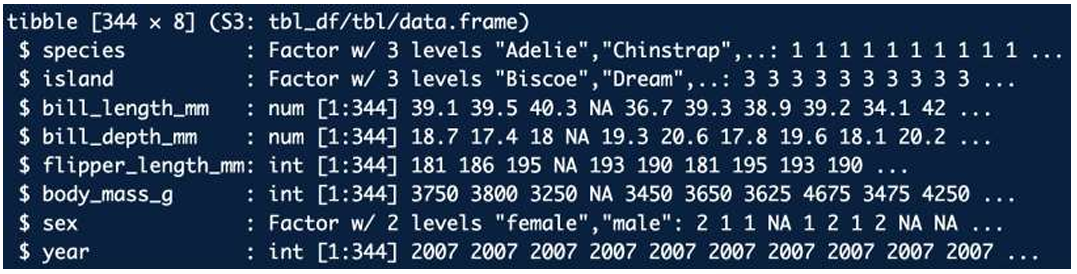
\includegraphics[width =\textwidth]{images/datasetPenguins.png}
\end{figure}